% Appendix A

\chapter{Implementatie en resultaten} % Main appendix title

\label{BijlageCode} 

\section{Docker-compose opstelling voor k6, InfluxDB \& Grafana}

\label{Bijlagek6}

Om de loadtest met k6, influxDB en grafana op te stellen heeft Loadimpact een docker-compose opstelling gemaakt. Na wat onderzoek is het opgevallen dat deze opstelling erg verouderd is. Daarom is ervoor gekozen om een eigen opstelling te maken:
\begin{minted}[linenos=true, bgcolor=codebg, breaklines]{yaml}
version: '3.4'

networks:
  k6:
  grafana:

services:
  influxdb:
    image: influxdb:1.5.4
    networks:
    - k6
    - grafana
    ports:
      - "8086:8086"
    environment:
      - INFLUXDB_DB=k6
    
  grafana:
    image: grafana/grafana:6.4.1
    networks:
      - grafana
    ports:
      - "3000:3000"
    environment:
      - GF_AUTH_ANONYMOUS_ORG_ROLE=Admin
      - GF_AUTH_ANONYMOUS_ENABLED=true
      - GF_AUTH_BASIC_ENABLED=false
    volumes:
      - ./grafana/datasource.yml:/etc/grafana/provisioning/datasources /datasource.yml
  
  k6:
    image: loadimpact/k6:0.25.1
    networks:
      - k6
    ports:
      - "6565:6565"
    environment:
      - K6_OUT=influxdb=http://influxdb:8086/k6
    volumes:
      - ../k6:/k6
\end{minted}

Hiervoor is een Pull-Request gemaakt naar loadimpact/k6 om dit te verbeteren. \texttt{https://github.com/loadimpact/k6/pull/1183} samen met de issue\\ \texttt{https://github.com/loadimpact/k6/issues/1182}. Hierin is te lezen wat precies de veranderingen waren. De maintainers van k6 waren blij met de verandering en hebben deze geaccepteerd en gemerged naar master. De loadtest is geschreven in javascript met de volgende code:
\begin{minted}[linenos=true, bgcolor=codebg, breaklines]{javascript}
import http from "k6/http";
import { sleep, check } from "k6";

export let options = {
  stages: [
    { duration: "10s", target: 20 },
    { duration: "10s", target: 40 },
    { duration: "10s", target: 60 },
    { duration: "10s", target: 80 },
    { duration: "10s", target: 100 },
    { duration: "10s", target: 120 },
  ]
};

export default function() {
  check(http.get("https://test.developers.nl/"), {
    "is status 200": (r) => r.status === 200
  });
  sleep(1);
};
\end{minted}

\section{k6 load test resultaten}

\label{bijlageloadtest}

In figuur \ref{fig:loadtestcli} is de CLI output van de loadtest te vinden. In figuur \ref{fig:loadtestvus} zijn de oplopende hoeveelheid VUs uitgebeeld in Grafana, en in figuur \ref{fig:loadtestresultaten} is in Grafana te zien hoe lang de requests duren.
\begin{figure}[H]
	\centering
	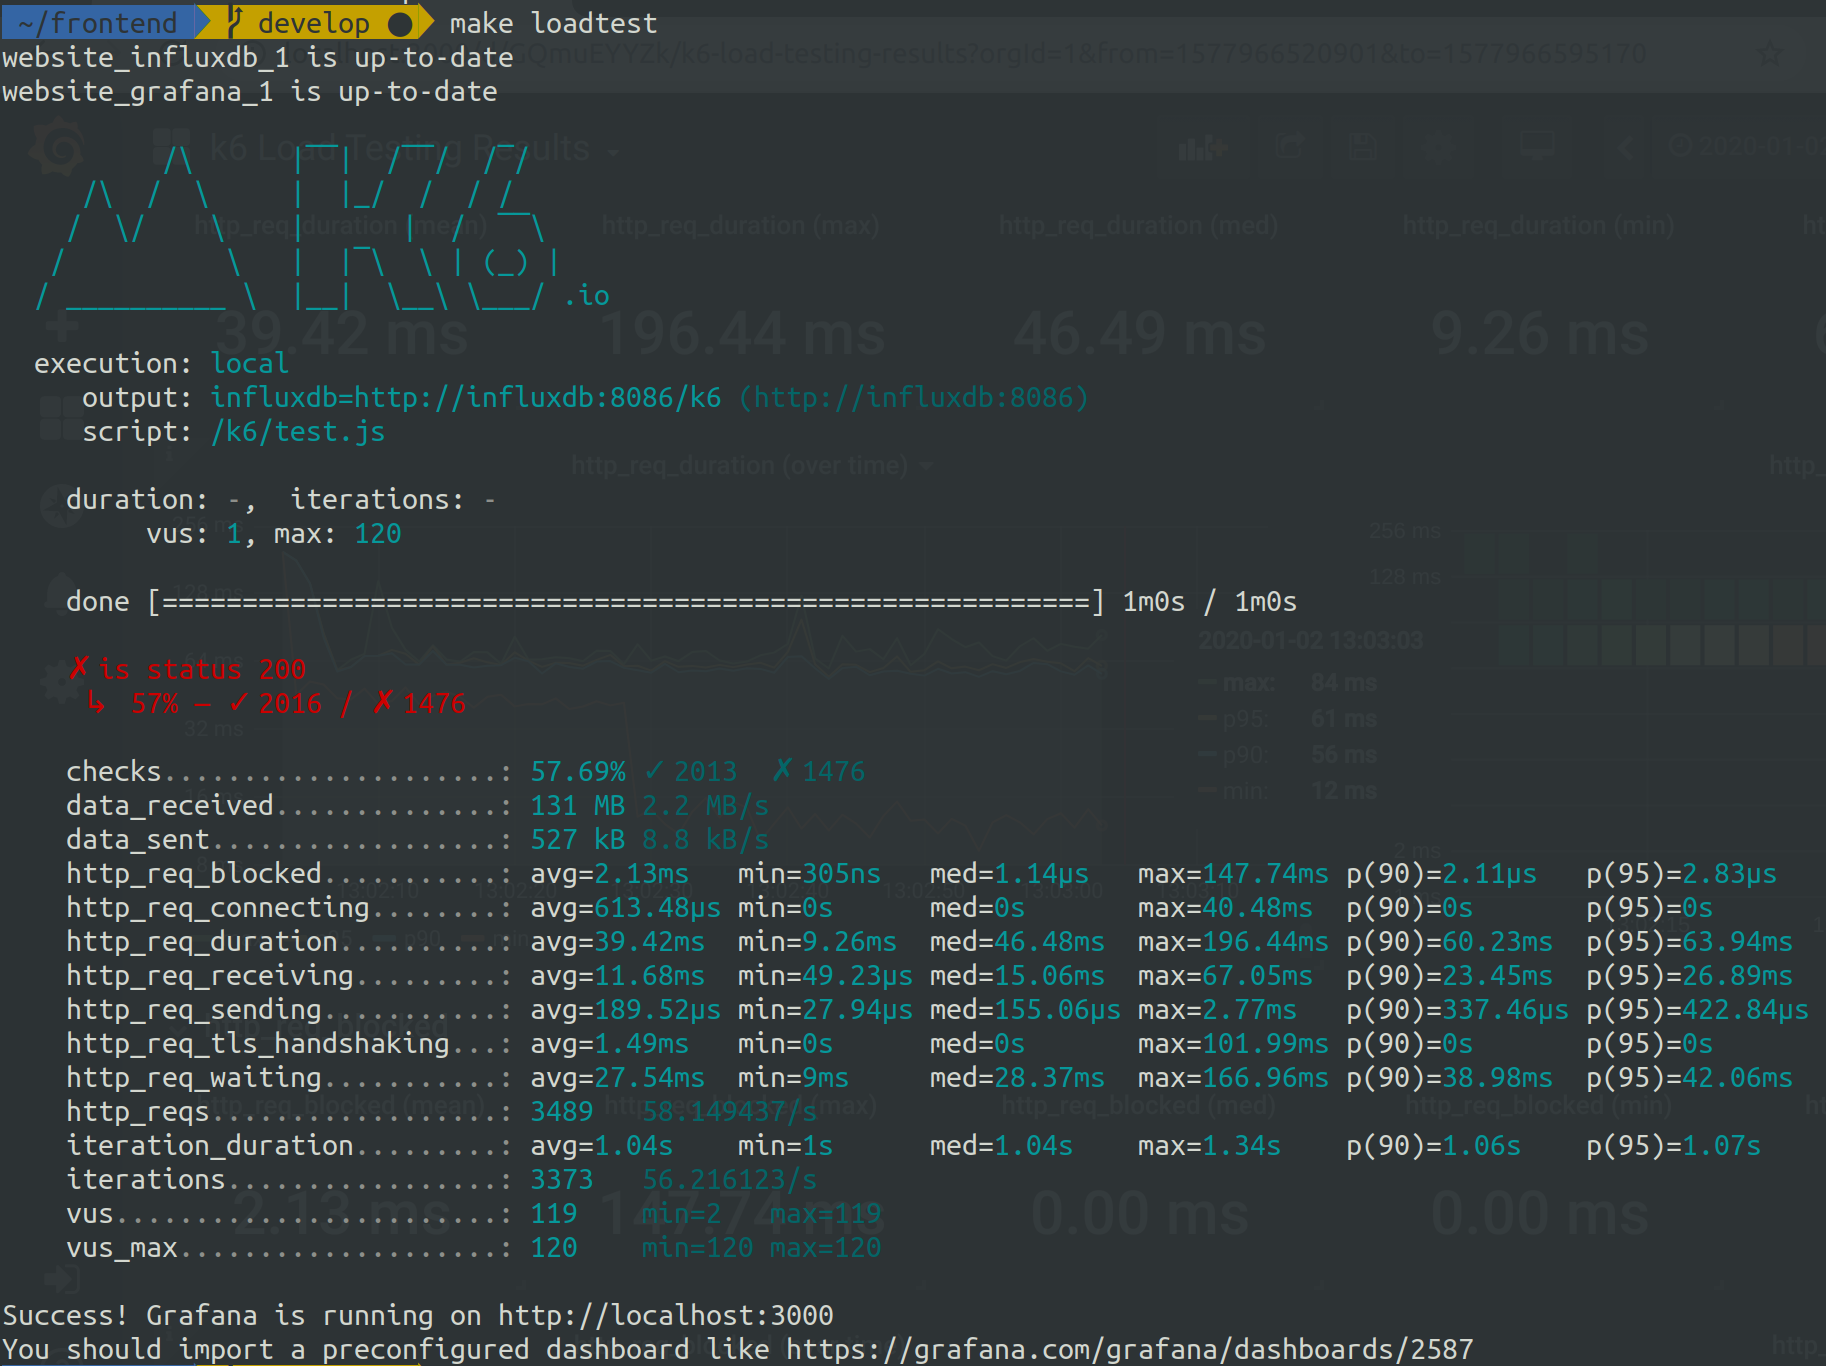
\includegraphics[width=13cm]{Figures/loadtest}
	\decoRule
	\caption[k6 loadtest CLI resultaten]{k6 loadtest CLI resultaten}
	\label{fig:loadtestcli}
\end{figure}

\begin{figure}[H]
	\centering
	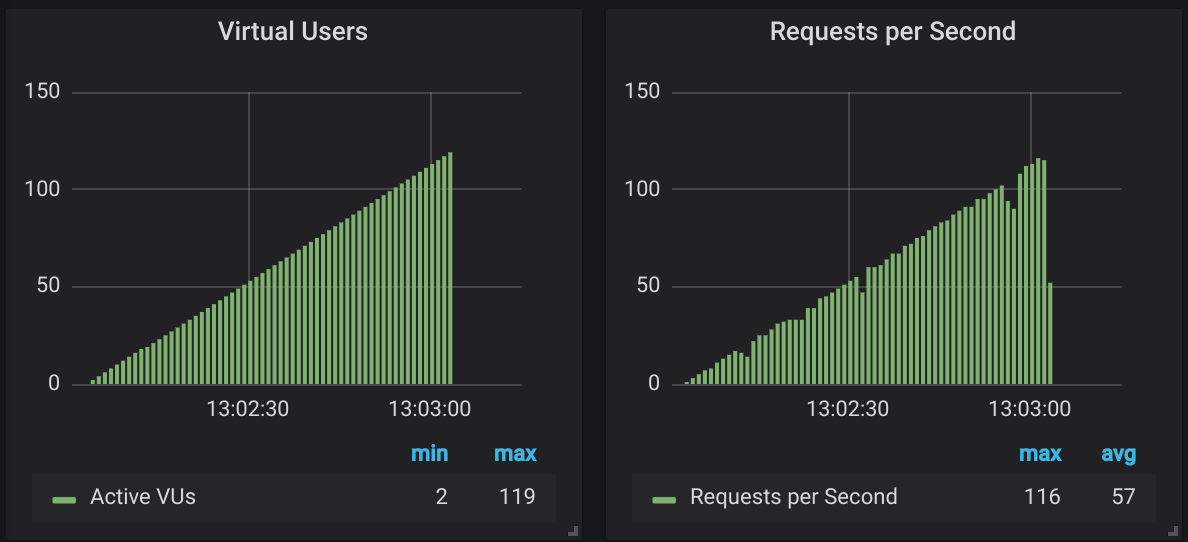
\includegraphics[width=13cm]{Figures/loadtestusers}
	\decoRule
	\caption[k6 loadtest hoeveelheid VUs en requests]{k6 loadtest hoeveelheid VUs en requests}
	\label{fig:loadtestvus}
\end{figure}

\begin{figure}[H]
	\centering
	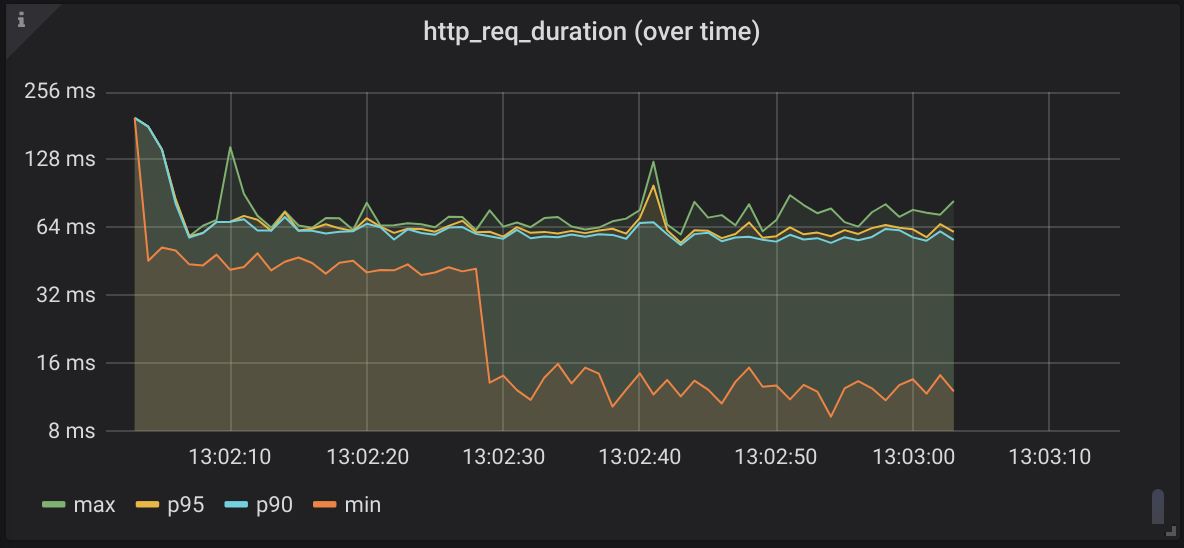
\includegraphics[width=13cm]{Figures/loadtestrequests}
	\decoRule
	\caption[k6 loadtest resultaten]{k6 loadtest resultaten}
	\label{fig:loadtestresultaten}
\end{figure}


\section{Docker container exits}

\label{DockerExits}

\subsubsection{PostgreSQL}
\begin{minted}[linenos=true, bgcolor=codebg, breaklines]{text}
LOG: received smart shutdown request
LOG: background worker "logical replication launcher" (PID 43) exited with exit code 1
LOG: shutting down
LOG: database system is shut down
\end{minted}

\subsubsection{PHP-FPM}
\begin{minted}[linenos=true, bgcolor=codebg, breaklines]{text}
NOTICE: Terminating ...
NOTICE: exiting, bye-bye!
\end{minted}

\subsubsection{Redis}
\begin{minted}[linenos=true, bgcolor=codebg, breaklines]{text}
1:signal-handler (1570781278) Received SIGTERM scheduling shutdown...
# User requested shutdown...
* Saving the final RDB snapshot before exiting.
* DB saved on disk
* Removing the pid file.
# Redis is now ready to exit, bye bye...
\end{minted}

\subsubsection{Nginx}
\begin{minted}[linenos=true, bgcolor=codebg, breaklines]{text}
[notice] 1#1: signal 15 (SIGTERM) received from 56, exiting
[notice] 48#48: exiting
[notice] 47#47: exiting
[notice] 47#47: exit
[notice] 1#1: signal 14 (SIGALRM) received
[notice] 1#1: signal 17 (SIGCHLD) received from 48
[notice] 1#1: cache manager process 48 exited with code 0
[notice] 1#1: worker process 47 exited with code 0
[notice] 1#1: exit
\end{minted}

\section{Docker container kill \& restarts}

\label{DockerKills}

\begin{minted}[linenos=true, bgcolor=codebg, breaklines]{text}
$ docker ps -q
d0829783af18
f72e9967771b
01dd48ff5a59
fab794731d47
ca510c065d11
3ee85578efb5

$ docker kill $(docker ps -q) 

$ docker ps
d0829783af18
f72e9967771b
01dd48ff5a59
fab794731d47
ca510c065d11
3ee85578efb5

$ docker ps -q

$ docker start $(docker ps -aq)
d0829783af18
f72e9967771b
01dd48ff5a59
fab794731d47
d68d7ab9809c
ca510c065d11
3ee85578efb5
e1866ab6c1af

$ docker ps -q
d0829783af18
f72e9967771b
01dd48ff5a59
fab794731d47
ca510c065d11
3ee85578efb5
\end{minted}

\section{Codecov implementatie} \label{codecov}
README.MD:
\begin{minted}[linenos=true, bgcolor=codebg, breaklines]{text}
## Tests

We enforce that code coverage stays acceptable using codecov:

[![codecov](https://codecov.io/bb/developers_nl/developers.nl/branch/ma
ster/graph/badge.svg?token=DzAv79t9Gd)](https://codecov.io/bb/developer
s_nl/developers.nl)
\end{minted}

Het builden van de Docker images met Ansible, inclusief de build arguments nodig voor codecov:
\begin{minted}[linenos=true, bgcolor=codebg, breaklines]{yaml}
docker_images:
  - dockerfile: docker/php7-fpm/Dockerfile
  path: ../
  name: developersnl/website-php-fpm
  buildargs:
    GROUP_ID: 9000
    USER_ID: 9000
    BITBUCKET_BRANCH: "{{ lookup('env','BITBUCKET_BRANCH') }}"
    BITBUCKET_COMMIT: "{{ lookup('env', 'BITBUCKET_COMMIT') }}"
    BITBUCKET_BUILD_NUMBER: "{{ lookup('env','BITBUCKET_BUILD_NUMBER') }}"
    BITBUCKET_REPO_OWNER: "{{ lookup('env','BITBUCKET_REPO_OWNER') }}"
    BITBUCKET_REPO_SLUG: "{{ lookup('env','BITBUCKET_REPO_SLUG') }}"
    BITBUCKET_PR_ID: "{{ lookup('env','BITBUCKET_PR_ID') }}"
    CODECOV_TOKEN: "{{ lookup('env','CODECOV_TOKEN') }}"
    CI: "{{ lookup('env','CI') }}"
\end{minted}

In de php7-fpm dockerfile zijn de build args omgezet naar environment variablen, een aantal apk packages toegevoegd en is het codecov script toegevoegd:
\begin{minted}[linenos=true, bgcolor=codebg, breaklines]{bash}
FROM application AS test

ENV SYMFONY_PHPUNIT_VERSION 8.0.0

ARG BITBUCKET_BRANCH
ARG BITBUCKET_BUILD_NUMBER
ARG BITBUCKET_REPO_OWNER
ARG BITBUCKET_REPO_SLUG
ARG BITBUCKET_PR_ID
ARG CODECOV_TOKEN
ARG CI
ARG BITBUCKET_COMMIT

ENV BITBUCKET_BRANCH=$BITBUCKET_BRANCH
ENV BITBUCKET_BUILD_NUMBER=$BITBUCKET_BUILD_NUMBER
ENV BITBUCKET_REPO_OWNER=$BITBUCKET_REPO_OWNER
ENV BITBUCKET_REPO_SLUG=$BITBUCKET_REPO_SLUG
ENV BITBUCKET_PR_ID=$BITBUCKET_PR_ID
ENV CODECOV_TOKEN=$CODECOV_TOKEN
ENV CI=$CI

# TODO: Cange VCS_COMMIT_ID to BITBUCKET_COMMIT when https://github.com/codecov/codecov-bash/pull/225 is deployed
ENV VCS_COMMIT_ID=$BITBUCKET_COMMIT

COPY --from=composer:1.9.0 /usr/bin/composer /usr/bin/composer

RUN apk add \
    php7-pdo_sqlite \
    php7-sqlite3 \
    php7-phar \
    php7-pear \
    php7-dev \
    redis \
    curl \
    bash \
    git \
    mercurial \
    findutils \
    g++ \
    make \
 && . /bin/pcov.sh \
 && redis-server --daemonize yes --requirepass test \
 && composer install -d /app/src --optimize-autoloader --no-interaction --no-suggest --no-scripts \
 && chmod u+x,g+x /app/src/bin/phpunit \
 && /app/src/bin/phpunit --configuration /app/src/phpunit.xml --coverage-clover=coverage.xml \
 && curl -s https://codecov.io/bash | bash -s - -X coveragepy
\end{minted}

pcov script:
\begin{minted}[linenos=true, bgcolor=codebg, breaklines]{bash}
#!/bin/sh

# Add PHP Coverage ini configuration
echo "- Enabling pcov"
cat <<-EOF > /etc/php7/conf.d/pcov.ini
extension=pcov
pcov.enable=1
EOF

echo "- Installing pcov"
if ! pecl list | grep pcov >/dev/null 2>&1;
then
    pecl install pcov ||
    {
        echo "Could not pecl install pcov" >&2;
        exit 1;
    }
fi
\end{minted}

\section{Feature-environments}
\begin{figure}[H]
	\centering
	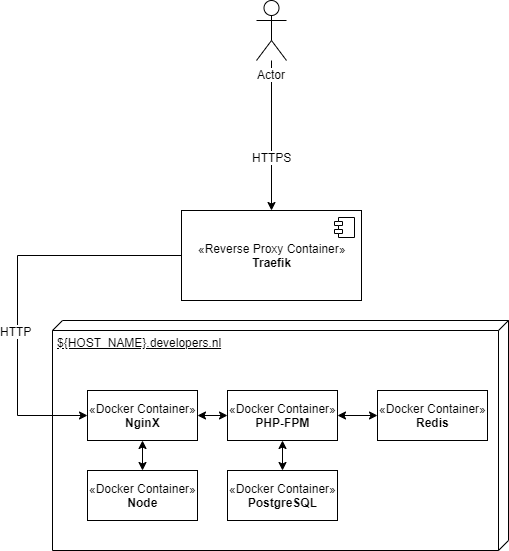
\includegraphics[width=13cm]{Figures/Traefik}
	\decoRule
	\caption[Traefik Infrastructure]{Nieuwe infrastructuur met Traefik reverse proxy}
	\label{fig:traefikinfrastructure}
\end{figure}
\begin{figure}[H]
	\centering
	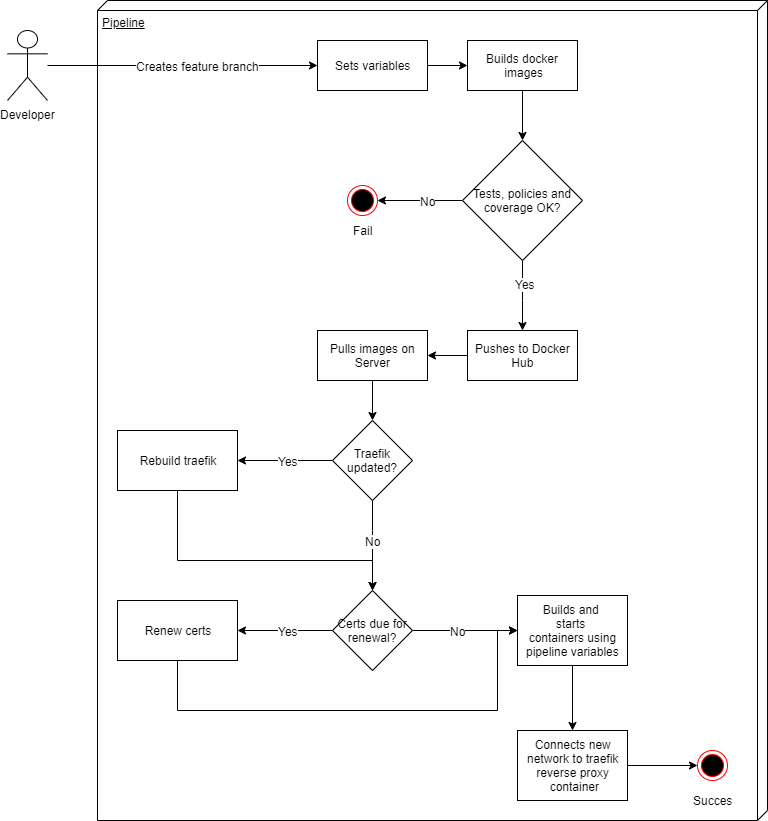
\includegraphics[width=13cm]{Figures/Activitydiagram}
	\decoRule
	\caption[Pipeline Activity Diagram]{Activity Diagram voor de pipeline}
	\label{fig:activitydiagram}
\end{figure}